\documentclass[a4paper]{article}
\usepackage{a4wide}
\usepackage[spanish,activeacute]{babel}
\usepackage{enumerate}
\usepackage{xspace}
\usepackage{longtable}
\usepackage{graphics}
\usepackage{listings}

\usepackage{calc}
\usepackage{lmodern}
\usepackage{amssymb}
\usepackage{amsmath}
\usepackage{mathdots}
\usepackage{mathtools}
\usepackage{multicol}
\usepackage{enumitem}
\usepackage{tasks}

\usepackage{ifthen}
\usepackage{amssymb}
\usepackage{multicol}
\usepackage{graphicx}
\usepackage[absolute]{textpos}
\usepackage{amsmath, amscd, amssymb, amsthm, latexsym}
% \usepackage[noload]{qtree}
%\usepackage{xspace,rotating,calligra,dsfont,ifthen}
\usepackage{xspace,rotating,dsfont,ifthen}
\usepackage[spanish,activeacute]{babel}
\usepackage[utf8]{inputenc}
\usepackage{pgfpages}
\usepackage{pgf,pgfarrows,pgfnodes,pgfautomata,pgfheaps,xspace,dsfont}
\usepackage{listings}
\usepackage{multicol}
\usepackage{todonotes}
\usepackage{url}
\usepackage{float}
\usepackage{framed,mdframed}
\usepackage{cancel}

\usepackage[strict]{changepage}


\makeatletter


\newcommand\hfrac[2]{\genfrac{}{}{0pt}{}{#1}{#2}} %\hfrac{}{} es un \frac sin la linea del medio

\newcommand\Wider[2][3em]{% \Wider[3em]{} reduce los m\'argenes
\makebox[\linewidth][c]{%
  \begin{minipage}{\dimexpr\textwidth+#1\relax}
  \raggedright#2
  \end{minipage}%
  }%
}


\@ifclassloaded{beamer}{%
  \newcommand{\tocarEspacios}{%
    \addtolength{\leftskip}{4em}%
    \addtolength{\parindent}{-3em}%
  }%
}
{%
  \usepackage[top=1cm,bottom=2cm,left=1cm,right=1cm]{geometry}%
  \usepackage{color}%
  \newcommand{\tocarEspacios}{%
    \addtolength{\leftskip}{3em}%
    \setlength{\parindent}{0em}%
  }%
}

\newcommand{\encabezadoDeProc}[4]{%
  % Ponemos la palabrita problema en tt
%  \noindent%
  {\normalfont\bfseries\ttfamily proc}%
  % Ponemos el nombre del problema
  \ %
  {\normalfont\ttfamily #2}%
  \
  % Ponemos los parametros
  (#3)%
  \ifthenelse{\equal{#4}{}}{}{%
  \ =\ %
  % Ponemos el nombre del resultado
  {\normalfont\ttfamily #1}%
  % Por ultimo, va el tipo del resultado
  \ : #4}
}

\newcommand{\encabezadoDeTipo}[2]{%
  % Ponemos la palabrita tipo en tt
  {\normalfont\bfseries\ttfamily tipo}%
  % Ponemos el nombre del tipo
  \ %
  {\normalfont\ttfamily #2}%
  \ifthenelse{\equal{#1}{}}{}{$\langle$#1$\rangle$}
}

% Primero definiciones de cosas al estilo title, author, date

\def\materia#1{\gdef\@materia{#1}}
\def\@materia{No especifi\'o la materia}
\def\lamateria{\@materia}

\def\cuatrimestre#1{\gdef\@cuatrimestre{#1}}
\def\@cuatrimestre{No especifi\'o el cuatrimestre}
\def\elcuatrimestre{\@cuatrimestre}

\def\anio#1{\gdef\@anio{#1}}
\def\@anio{No especifi\'o el anio}
\def\elanio{\@anio}

\def\fecha#1{\gdef\@fecha{#1}}
\def\@fecha{\today}
\def\lafecha{\@fecha}

\def\nombre#1{\gdef\@nombre{#1}}
\def\@nombre{No especific'o el nombre}
\def\elnombre{\@nombre}

\def\practicas#1{\gdef\@practica{#1}}
\def\@practica{No especifi\'o el n\'umero de pr\'actica}
\def\lapractica{\@practica}


% Esta macro convierte el numero de cuatrimestre a palabras
\newcommand{\cuatrimestreLindo}{
  \ifthenelse{\equal{\elcuatrimestre}{1}}
  {Primer cuatrimestre}
  {\ifthenelse{\equal{\elcuatrimestre}{2}}
  {Segundo cuatrimestre}
  {Verano}}
}


\newcommand{\depto}{{UBA -- Facultad de Ciencias Exactas y Naturales --
      Departamento de Computaci\'on}}

\newcommand{\titulopractica}{
  \centerline{\depto}
  \vspace{1ex}
  \centerline{{\Large\lamateria}}
  \vspace{0.5ex}
  \centerline{\cuatrimestreLindo de \elanio}
  \vspace{2ex}
  \centerline{{\huge Pr\'actica \lapractica -- \elnombre}}
  \vspace{5ex}
  \arreglarincisos
  \newcounter{ejercicio}
  \newenvironment{ejercicio}{\stepcounter{ejercicio}\textbf{Ejercicio
      \theejercicio}%
    \renewcommand\@currentlabel{\theejercicio}%
  }{\vspace{0.2cm}}
}


\newcommand{\titulotp}{
  \centerline{\depto}
  \vspace{1ex}
  \centerline{{\Large\lamateria}}
  \vspace{0.5ex}
  \centerline{\cuatrimestreLindo de \elanio}
  \vspace{0.5ex}
  \centerline{\lafecha}
  \vspace{2ex}
  \centerline{{\huge\elnombre}}
  \vspace{5ex}
}


%practicas
\newcommand{\practica}[2]{%
    \title{Pr\'actica #1 \\ #2}
    \author{Algoritmos y Estructuras de Datos I}
    \date{Segundo Cuatrimestre 2019}

    \maketitlepractica{#1}{#2}
}

\newcommand \maketitlepractica[2] {%
\begin{center}
\begin{tabular}{r cr}
 \begin{tabular}{c}
{\large\bf\textsf{\ Algoritmos y Estructuras de Datos I\ }}\\
Primer Cuatrimestre 2020\\
\title{\normalsize Gu\'ia Pr\'actica #1 \\ \textbf{#2}}\\
\@title
\end{tabular} &
\begin{tabular}{@{} p{1.6cm} @{}}

\includegraphics[width=1.6cm]{logodpt.jpg}
\end{tabular} &
\begin{tabular}{l @{}}
 \emph{Departamento de Computaci\'on} \\
 \emph{Facultad de Ciencias Exactas y Naturales} \\
 \emph{Universidad de Buenos Aires} \\
\end{tabular}
\end{tabular}
\end{center}

\bigskip
}


% Símbolos varios

\newcommand{\nat}{\ensuremath{\mathds{N}}}
\newcommand{\ent}{\ensuremath{\mathds{Z}}}
\newcommand{\float}{\ensuremath{\mathds{R}}}
\newcommand{\bool}{\ensuremath{\mathsf{Bool}}}
\newcommand{\True}{\ensuremath{\mathrm{true}}}
\newcommand{\False}{\ensuremath{\mathrm{false}}}
\newcommand{\Then}{\ensuremath{\rightarrow}}
\newcommand{\Iff}{\ensuremath{\leftrightarrow}}
\newcommand{\implica}{\ensuremath{\longrightarrow}}
\newcommand{\IfThenElse}[3]{\ensuremath{\mathsf{if}\ #1\ \mathsf{then}\ #2\ \mathsf{else}\ #3\ \mathsf{fi}}}
\newcommand{\In}{\textsf{in }}
\newcommand{\Out}{\textsf{out }}
\newcommand{\Inout}{\textsf{inout }}
\newcommand{\yLuego}{\land _L}
\newcommand{\oLuego}{\lor _L}
\newcommand{\implicaLuego}{\implica _L}
\newcommand{\cuantificador}[5]{%
	\ensuremath{(#2 #3: #4)\ (%
		\ifthenelse{\equal{#1}{unalinea}}{
			#5
		}{
			$ % exiting math mode
			\begin{adjustwidth}{+2em}{}
			$#5$%
			\end{adjustwidth}%
			$ % entering math mode
		}
	)}
}

\newcommand{\existe}[4][]{%
	\cuantificador{#1}{\exists}{#2}{#3}{#4}
}
\newcommand{\paraTodo}[4][]{%
	\cuantificador{#1}{\forall}{#2}{#3}{#4}
}

% Símbolo para marcar los ejercicios importantes (estrellita)
\newcommand\importante{\raisebox{0.5pt}{\ensuremath{\bigstar}}}


\newcommand{\rango}[2]{[#1\twodots#2]}
\newcommand{\comp}[2]{[\,#1\,|\,#2\,]}

\newcommand{\rangoac}[2]{(#1\twodots#2]}
\newcommand{\rangoca}[2]{[#1\twodots#2)}
\newcommand{\rangoaa}[2]{(#1\twodots#2)}

%ejercicios
\newtheorem{exercise}{Ejercicio}
\newenvironment{ejercicio}[1][]{\begin{exercise}#1\rm}{\end{exercise} \vspace{0.2cm}}
\newenvironment{items}{\begin{enumerate}[a)]}{\end{enumerate}}
\newenvironment{subitems}{\begin{enumerate}[i)]}{\end{enumerate}}
\newcommand{\sugerencia}[1]{\noindent \textbf{Sugerencia:} #1}

\lstnewenvironment{code}{
    \lstset{% general command to set parameter(s)
        language=C++, basicstyle=\small\ttfamily, keywordstyle=\slshape,
        emph=[1]{tipo,usa}, emphstyle={[1]\sffamily\bfseries},
        morekeywords={tint,forn,forsn},
        basewidth={0.47em,0.40em},
        columns=fixed, fontadjust, resetmargins, xrightmargin=5pt, xleftmargin=15pt,
        flexiblecolumns=false, tabsize=2, breaklines, breakatwhitespace=false, extendedchars=true,
        numbers=left, numberstyle=\tiny, stepnumber=1, numbersep=9pt,
        frame=l, framesep=3pt,
    }
   \csname lst@SetFirstLabel\endcsname}
  {\csname lst@SaveFirstLabel\endcsname}


%tipos basicos
\newcommand{\rea}{\ensuremath{\mathsf{Float}}}
\newcommand{\cha}{\ensuremath{\mathsf{Char}}}
\newcommand{\str}{\ensuremath{\mathsf{String}}}

\newcommand{\mcd}{\mathrm{mcd}}
\newcommand{\prm}[1]{\ensuremath{\mathsf{prm}(#1)}}
\newcommand{\sgd}[1]{\ensuremath{\mathsf{sgd}(#1)}}

\newcommand{\tuple}[2]{\ensuremath{#1 \times #2}}

%listas
\newcommand{\TLista}[1]{\ensuremath{seq \langle #1\rangle}}
\newcommand{\lvacia}{\ensuremath{[\ ]}}
\newcommand{\lv}{\ensuremath{[\ ]}}
\newcommand{\longitud}[1]{\ensuremath{|#1|}}
\newcommand{\cons}[1]{\ensuremath{\mathsf{addFirst}}(#1)}
\newcommand{\indice}[1]{\ensuremath{\mathsf{indice}}(#1)}
\newcommand{\conc}[1]{\ensuremath{\mathsf{concat}}(#1)}
\newcommand{\cab}[1]{\ensuremath{\mathsf{head}}(#1)}
\newcommand{\cola}[1]{\ensuremath{\mathsf{tail}}(#1)}
\newcommand{\sub}[1]{\ensuremath{\mathsf{subseq}}(#1)}
\newcommand{\en}[1]{\ensuremath{\mathsf{en}}(#1)}
\newcommand{\cuenta}[2]{\mathsf{cuenta}\ensuremath{(#1, #2)}}
\newcommand{\suma}[1]{\mathsf{suma}(#1)}
\newcommand{\twodots}{\ensuremath{\mathrm{..}}}
\newcommand{\masmas}{\ensuremath{++}}
\newcommand{\matriz}[1]{\TLista{\TLista{#1}}}

% Acumulador
\newcommand{\acum}[1]{\ensuremath{\mathsf{acum}}(#1)}
\newcommand{\acumselec}[3]{\ensuremath{\mathrm{acum}(#1 |  #2, #3)}}

% \selector{variable}{dominio}
\newcommand{\selector}[2]{#1~\ensuremath{\leftarrow}~#2}
\newcommand{\selec}{\ensuremath{\leftarrow}}

\newcommand{\pred}[3]{%
    {\normalfont\bfseries\ttfamily\noindent pred }%
    {\normalfont\ttfamily #1}%
    \ifthenelse{\equal{#2}{}}{}{\ (#2) }%
    \{%
    \begin{adjustwidth}{+2em}{}
      \ensuremath{#3}
    \end{adjustwidth}
    \}%
    {\normalfont\bfseries\,\par}%
}

\newenvironment{proc}[4][res]{%

  % El parametro 1 (opcional) es el nombre del resultado
  % El parametro 2 es el nombre del problema
  % El parametro 3 son los parametros
  % El parametro 4 es el tipo del resultado
  % Preambulo del ambiente problema
  % Tenemos que definir los comandos requiere, asegura, modifica y aux
  \newcommand{\pre}[2][]{%
    {\normalfont\bfseries\ttfamily Pre}%
    \ifthenelse{\equal{##1}{}}{}{\ {\normalfont\ttfamily ##1} :}\ %
    \{\ensuremath{##2}\}%
    {\normalfont\bfseries\,\par}%
  }
  \newcommand{\post}[2][]{%
    {\normalfont\bfseries\ttfamily Post}%
    \ifthenelse{\equal{##1}{}}{}{\ {\normalfont\ttfamily ##1} :}\
    \{\ensuremath{##2}\}%
    {\normalfont\bfseries\,\par}%
  }
  \renewcommand{\aux}[4]{%
    {\normalfont\bfseries\ttfamily aux\ }%
    {\normalfont\ttfamily ##1}%
    \ifthenelse{\equal{##2}{}}{}{\ (##2)}\ : ##3\, = \ensuremath{##4}%
    {\normalfont\bfseries\,;\par}%
  }
  \renewcommand{\pred}[3]{%
    {\normalfont\bfseries\ttfamily pred }%
    {\normalfont\ttfamily ##1}%
    \ifthenelse{\equal{##2}{}}{}{\ (##2) }%
    \{%
    \begin{adjustwidth}{+5em}{}
      \ensuremath{##3}
    \end{adjustwidth}
    \}%
    {\normalfont\bfseries\,\par}%
  }

  \newcommand{\res}{#1}
  \vspace{1ex}
  \noindent
  \encabezadoDeProc{#1}{#2}{#3}{#4}
  % Abrimos la llave
  \{\par%
  \tocarEspacios
}
% Ahora viene el cierre del ambiente problema
{
  % Cerramos la llave
  \noindent\}
  \vspace{1ex}
}


\newcommand{\aux}[4]{%
    {\normalfont\bfseries\ttfamily\noindent aux\ }%
    {\normalfont\ttfamily #1}%
    \ifthenelse{\equal{#2}{}}{}{\ (#2)}\ : #3\, = \ensuremath{#4}%
    {\normalfont\bfseries\,;\par}%
}


% \newcommand{\pre}[1]{\textsf{pre}\ensuremath{(#1)}}

\newcommand{\procnom}[1]{\textsf{#1}}
\newcommand{\procil}[3]{\textsf{proc #1}\ensuremath{(#2) = #3}}
\newcommand{\procilsinres}[2]{\textsf{proc #1}\ensuremath{(#2)}}
\newcommand{\preil}[2]{\textsf{Pre #1: }\ensuremath{#2}}
\newcommand{\postil}[2]{\textsf{Post #1: }\ensuremath{#2}}
\newcommand{\auxil}[2]{\textsf{fun }\ensuremath{#1 = #2}}
\newcommand{\auxilc}[4]{\textsf{fun }\ensuremath{#1( #2 ): #3 = #4}}
\newcommand{\auxnom}[1]{\textsf{fun }\ensuremath{#1}}
\newcommand{\auxpred}[3]{\textsf{pred }\ensuremath{#1( #2 ) \{ #3 \}}}

\newcommand{\comentario}[1]{{/*\ #1\ */}}

\newcommand{\nom}[1]{\ensuremath{\mathsf{#1}}}


% En las practicas/parciales usamos numeros arabigos para los ejercicios.
% Aca cambiamos los enumerate comunes para que usen letras y numeros
% romanos
\newcommand{\arreglarincisos}{%
  \renewcommand{\theenumi}{\alph{enumi}}
  \renewcommand{\theenumii}{\roman{enumii}}
  \renewcommand{\labelenumi}{\theenumi)}
  \renewcommand{\labelenumii}{\theenumii)}
}



%%%%%%%%%%%%%%%%%%%%%%%%%%%%%% PARCIAL %%%%%%%%%%%%%%%%%%%%%%%%
\let\@xa\expandafter
\newcommand{\tituloparcial}{\centerline{\depto -- \lamateria}
  \centerline{\elnombre -- \lafecha}%
  \setlength{\TPHorizModule}{10mm} % Fija las unidades de textpos
  \setlength{\TPVertModule}{\TPHorizModule} % Fija las unidades de
                                % textpos
  \arreglarincisos
  \newcounter{total}% Este contador va a guardar cuantos incisos hay
                    % en el parcial. Si un ejercicio no tiene incisos,
                    % cuenta como un inciso.
  \newcounter{contgrilla} % Para hacer ciclos
  \newcounter{columnainicial} % Se van a usar para los cline cuando un
  \newcounter{columnafinal}   % ejercicio tenga incisos.
  \newcommand{\primerafila}{}
  \newcommand{\segundafila}{}
  \newcommand{\rayitas}{} % Esto va a guardar los \cline de los
                          % ejercicios con incisos, asi queda mas bonito
  \newcommand{\anchodegrilla}{20} % Es para textpos
  \newcommand{\izquierda}{7} % Estos dos le dicen a textpos donde colocar
  \newcommand{\abajo}{2}     % la grilla
  \newcommand{\anchodecasilla}{0.4cm}
  \setcounter{columnainicial}{1}
  \setcounter{total}{0}
  \newcounter{ejercicio}
  \setcounter{ejercicio}{0}
  \renewenvironment{ejercicio}[1]
  {%
    \stepcounter{ejercicio}\textbf{\noindent Ejercicio \theejercicio. [##1
      puntos]}% Formato
    \renewcommand\@currentlabel{\theejercicio}% Esto es para las
                                % referencias
    \newcommand{\invariante}[2]{%
      {\normalfont\bfseries\ttfamily invariante}%
      \ ####1\hspace{1em}####2%
    }%
    \newcommand{\Proc}[5][result]{
      \encabezadoDeProc{####1}{####2}{####3}{####4}\hspace{1em}####5}%
  }% Aca se termina el principio del ejercicio
  {% Ahora viene el final
    % Esto suma la cantidad de incisos o 1 si no hubo ninguno
    \ifthenelse{\equal{\value{enumi}}{0}}
    {\addtocounter{total}{1}}
    {\addtocounter{total}{\value{enumi}}}
    \ifthenelse{\equal{\value{ejercicio}}{1}}{}
    {
      \g@addto@macro\primerafila{&} % Si no estoy en el primer ej.
      \g@addto@macro\segundafila{&}
    }
    \ifthenelse{\equal{\value{enumi}}{0}}
    {% No tiene incisos
      \g@addto@macro\primerafila{\multicolumn{1}{|c|}}
      \bgroup% avoid overwriting somebody else's value of \tmp@a
      \protected@edef\tmp@a{\theejercicio}% expand as far as we can
      \@xa\g@addto@macro\@xa\primerafila\@xa{\tmp@a}%
      \egroup% restore old value of \tmp@a, effect of \g@addto.. is

      \stepcounter{columnainicial}
    }
    {% Tiene incisos
      % Primero ponemos el encabezado
      \g@addto@macro\primerafila{\multicolumn}% Ahora el numero de items
      \bgroup% avoid overwriting somebody else's value of \tmp@a
      \protected@edef\tmp@a{\arabic{enumi}}% expand as far as we can
      \@xa\g@addto@macro\@xa\primerafila\@xa{\tmp@a}%
      \egroup% restore old value of \tmp@a, effect of \g@addto.. is
      % global
      % Ahora el formato
      \g@addto@macro\primerafila{{|c|}}%
      % Ahora el numero de ejercicio
      \bgroup% avoid overwriting somebody else's value of \tmp@a
      \protected@edef\tmp@a{\theejercicio}% expand as far as we can
      \@xa\g@addto@macro\@xa\primerafila\@xa{\tmp@a}%
      \egroup% restore old value of \tmp@a, effect of \g@addto.. is
      % global
      % Ahora armamos la segunda fila
      \g@addto@macro\segundafila{\multicolumn{1}{|c|}{a}}%
      \setcounter{contgrilla}{1}
      \whiledo{\value{contgrilla}<\value{enumi}}
      {%
        \stepcounter{contgrilla}
        \g@addto@macro\segundafila{&\multicolumn{1}{|c|}}
        \bgroup% avoid overwriting somebody else's value of \tmp@a
        \protected@edef\tmp@a{\alph{contgrilla}}% expand as far as we can
        \@xa\g@addto@macro\@xa\segundafila\@xa{\tmp@a}%
        \egroup% restore old value of \tmp@a, effect of \g@addto.. is
        % global
      }
      % Ahora armo las rayitas
      \setcounter{columnafinal}{\value{columnainicial}}
      \addtocounter{columnafinal}{-1}
      \addtocounter{columnafinal}{\value{enumi}}
      \bgroup% avoid overwriting somebody else's value of \tmp@a
      \protected@edef\tmp@a{\noexpand\cline{%
          \thecolumnainicial-\thecolumnafinal}}%
      \@xa\g@addto@macro\@xa\rayitas\@xa{\tmp@a}%
      \egroup% restore old value of \tmp@a, effect of \g@addto.. is
      \setcounter{columnainicial}{\value{columnafinal}}
      \stepcounter{columnainicial}
    }
    \setcounter{enumi}{0}%
    \vspace{0.2cm}%
  }%
  \newcommand{\tercerafila}{}
  \newcommand{\armartercerafila}{
    \setcounter{contgrilla}{1}
    \whiledo{\value{contgrilla}<\value{total}}
    {\stepcounter{contgrilla}\g@addto@macro\tercerafila{&}}
  }
  \newcommand{\grilla}{%
    \g@addto@macro\primerafila{&\textbf{TOTAL}}
    \g@addto@macro\segundafila{&}
    \g@addto@macro\tercerafila{&}
    \armartercerafila
    \ifthenelse{\equal{\value{total}}{\value{ejercicio}}}
    {% No hubo incisos
      \begin{textblock}{\anchodegrilla}(\izquierda,\abajo)
        \begin{tabular}{|*{\value{total}}{p{\anchodecasilla}|}c|}
          \hline
          \primerafila\\
          \hline
          \tercerafila\\
          \tercerafila\\
          \hline
        \end{tabular}
      \end{textblock}
    }
    {% Hubo incisos
      \begin{textblock}{\anchodegrilla}(\izquierda,\abajo)
        \begin{tabular}{|*{\value{total}}{p{\anchodecasilla}|}c|}
          \hline
          \primerafila\\
          \rayitas
          \segundafila\\
          \hline
          \tercerafila\\
          \tercerafila\\
          \hline
        \end{tabular}
      \end{textblock}
    }
  }%
  \vspace{0.4cm}
  \textbf{Nro. de orden:}

  \textbf{LU:}

  \textbf{Apellidos:}

  \textbf{Nombres:}

  \textbf{Nro. de hojas que adjunta:}
  \vspace{0.5cm}
}



% AMBIENTE CONSIGNAS
% Se usa en el TP para ir agregando las cosas que tienen que resolver
% los alumnos.
% Dentro del ambiente hay que usar \item para cada consigna

\newcounter{consigna}
\setcounter{consigna}{0}

\newenvironment{consignas}{%
  \newcommand{\consigna}{\stepcounter{consigna}\textbf{\theconsigna.}}%
  \renewcommand{\ejercicio}[1]{\item ##1 }
  \renewcommand{\proc}[5][result]{\item
    \encabezadoDeProc{##1}{##2}{##3}{##4}\hspace{1em}##5}%
  \newcommand{\invariante}[2]{\item%
    {\normalfont\bfseries\ttfamily invariante}%
    \ ##1\hspace{1em}##2%
  }
  \renewcommand{\aux}[4]{\item%
    {\normalfont\bfseries\ttfamily aux\ }%
    {\normalfont\ttfamily ##1}%
    \ifthenelse{\equal{##2}{}}{}{\ (##2)}\ : ##3 \hspace{1em}##4%
  }
  % Comienza la lista de consignas
  \begin{list}{\consigna}{%
      \setlength{\itemsep}{0.5em}%
      \setlength{\parsep}{0cm}%
    }
}%
{\end{list}}



% para decidir si usar && o ^
\newcommand{\y}[0]{\ensuremath{\land}}

% macros de correctitud
\newcommand{\semanticComment}[2]{#1 \ensuremath{#2};}
\newcommand{\namedSemanticComment}[3]{#1 #2: \ensuremath{#3};}


\newcommand{\local}[1]{\semanticComment{local}{#1}}

\newcommand{\vale}[1]{\semanticComment{vale}{#1}}
\newcommand{\valeN}[2]{\namedSemanticComment{vale}{#1}{#2}}
\newcommand{\impl}[1]{\semanticComment{implica}{#1}}
\newcommand{\implN}[2]{\namedSemanticComment{implica}{#1}{#2}}
\newcommand{\estado}[1]{\semanticComment{estado}{#1}}

\newcommand{\invarianteCN}[2]{\namedSemanticComment{invariante}{#1}{#2}}
\newcommand{\invarianteC}[1]{\semanticComment{invariante}{#1}}
\newcommand{\varianteCN}[2]{\namedSemanticComment{variante}{#1}{#2}}
\newcommand{\varianteC}[1]{\semanticComment{variante}{#1}}




\begin{document}

\practica{2}{Introducción al Lenguaje de Especificación Resuelto}

\subsection*{Comentarios:}
Hola, este no es un resuelto oficial, tiene el logo del DC porque me parecio divertido copiar el formato de la guia.\\
\section{Secuencias}

\paragraph{\textbf{Ejercicio 1.}} $\bigstar $ Evaluar las siguientes expresiones:

\begin{multicols}{2}
\begin{enumerate}[label=\alph*)]
\item $ \vert \langle 4,3,1\rangle \vert$
\item addFirst$(\pi,\langle 2,3,5,7,11\rangle )$
\item $\langle 0,1,2,3\rangle [3]$
\item concat$(\langle 2,3\rangle ,\langle 5,7,11\rangle )$
\item head(tail$(\langle 5,6,7,8\rangle))$
\item subseq$(\langle 2,3,5,7,11\rangle ,0,3)$
\item $\pi \in \langle 2,3,5,7,11\rangle$
\item subseq$(\langle 2,3,5,7,11\rangle ,3,2)$
\item $1\in \langle 1,2,3,4,5\rangle$
\item subseq$(\langle 2,3,5,7,11\rangle , 0,65536)$
\end{enumerate} 
\end{multicols}

\subsection*{Respuestas}

\begin{multicols}{2}
\begin{enumerate}[label=\alph*)]
\item $3$
\item $\langle \pi,2,3,5,7,11\rangle$
\item $3$
\item $\langle 2,3,5,7,11\rangle$
\item $6$
\item $\langle 2,3,5 \rangle$
\item $False$
\item $\perp$
\item $True$
\item $\perp$
\end{enumerate}
\end{multicols}

\paragraph{\textbf{Ejercicio 2.}} $\bigstar $ Sea $x$ de tipo seq$\langle \mathbb{Z}\rangle$.¿Cuáles de las siguientes igualdades sobre secuencias son válidas?

\begin{multicols}{2}
\begin{enumerate}[label=\alph*)]
\item $\vert x\vert =\vert $tail$(x)\vert +1$
\item $x=$subseq$(x,0,\vert x \vert -1)$
\item $x=$subseq$(x,0,\vert x \vert )$
\item concat(addFirst$(3,x),y)=$ addFirst$(3,$concat$(x,y))$
\item $x=$ addFirst(head$(x),$tail$(x)$)
\item $x[0]=$ head$(x)$
\item $i \in x=\textrm{head(subseq}(x,i,i+1))$
\item $\textrm{tail}(x)=\textrm{subseq}(x,1,\vert x \vert )$
\end{enumerate}
\end{multicols}
En los casos incorrectos, ¿puede dar condiciones sobre las listas en cuestión para que lo sean?
\subsection*{Respuesta}
\begin{multicols}{2}
\begin{enumerate}[label=\alph*)]
\item Invalida, funciona con $x \neq \langle \rangle$ 
\item Invalida
\item Valida
\item Invalida, funciona con $y$ de tipo seq$\langle \mathbb{Z}\rangle$
\item Invalida, funciona con $x \neq \langle \rangle$
\item Invalida, funciona con $x \neq \langle \rangle$
\item Invalida
\item Invalida, funciona con $x \neq \langle \rangle$
\end{enumerate}
\end{multicols}

\paragraph{Ejercicio 3.} $\bigstar$ Sea $s_0,s_1$ secuencias de tipo $T$ y $e$ un elemento de tipo $T$. Indicar para cada una de las siguientes si son verdaderas o falsas. En caso de ser falsa, mostrar un contraejemplo.

\begin{enumerate}[label=\alph*)]
\item $\vert \textrm{addFirst}(e,s_0)\vert =1+ \vert s_0\vert$
\item $\vert \textrm{addFirst}(e,s_0)\vert = \vert \textrm{tail}(s_0)\vert $
\item $\vert \textrm{concat}(s_0,s_1)\vert = \vert s_0 \vert +\vert s_1\vert $
\item $s_0 = \textrm{tail(addFirst}(e,s_0))$
\item $\textrm{head(addFirst}(e,s_0))=e$
\item $\textrm{addFirst}(e,s_0)=\textrm{tail}(s_0)$
\item $\textrm{head(addFirst}(e,\textrm{tail}(s_0)))=\textrm{head(tail(addFirst}(e,s_0)))$
\item $\textrm{addFirst}(e,s_0)[0]=e$
\item $\textrm{addFirst}(e,s_0)[0]=\textrm{head(addFirst}(e,s_0))$
\end{enumerate}

\subsection*{Respuestas}

\begin{enumerate}[label=\alph*)]
\item $True$
\item $False$ $e=1;$ $s_0=\langle 2\rangle ;$ $s_1=\langle 3\rangle ;\rightarrow$  $2=0$
\item $True$
\item $True$
\item $True$
\item $False$ $e=1;$ $s_0=\langle 2\rangle ;$ $s_1=\langle 3\rangle ;\rightarrow$  $\langle 1,2\rangle =\langle \rangle$
\item $False$ $e=1;$ $s_0=\langle 2\rangle ;$ $s_1=\langle 3\rangle ;\rightarrow$  $ 1 = 2$
\item $True$
\item $True$
\end{enumerate}

\paragraph{Ejercicio 4.} $\bigstar$ Escriba los siguientes predicados auxiliares sobre secuencias de enteros, aclarando los tipos de los parámetros que recibe:

\begin{enumerate}[label=\alph*)]
\item $estaAcotada,$ que determina si todos los elementos de una sequencia están dentro del rango $[1,100]$.
\item $capicua,$ que es verdadera sii una secuencia es capicúa. (Por ejemplo, $\langle 0,2,1,2,0 \rangle$ es capicúa y $\langle 0,2,1,4,0\rangle$ no).
\item $esPrefijo,$ que es verdadera sii una secuencia es prefijo de otra.
\item $estaOrdenada,$ que es verdadera sii la secuencia está ordenada de menor a mayor.
\item $todosPrimos,$ que es verdadera sii todos los elementos de la secuencia son números primos.
\item $primosEnPosicionesPares,$ que es verdadero sii todos los elementos primos de una secuencia están de una posición par.
\item $todosIguales,$ que es verdadera sii todos los elemntos de la secuencia son iguales.
\item $hayUnParQueDivideAlResto,$ que determina si hay un elemento par en la secuencia que divide a todos los otros elementos de la secuencia.
\item $hayUnoEnPosicionParQueDivideAlResto,$ que determina si hay un elemento en una posición par de la secuencia que divide a todos los otros elementos contenidos en la secuencia.
\item $sinRepetidos,$ que determina si la secuencia no tiene repetidos.
\item $otroMayorADerecha,$ que determina si todo elemento de la secuencia, salvo el último, tiene otro mayor a su derecha.
\item $todoEsMultiplo,$ que determina si todo elemento de la secuencia es múltiplo de algún otro.
\item $enTresPartes,$ que determina si en la secuencia aparecen (de izquierda a derecha) primero 0s, después 1s y por último 2s. Por ejemplo $\langle 0,0,1,1,1,1,2\rangle$ cumple con $enTresPartes,$ pero $\langle 0,1,3,0\rangle$ o $\langle 0,0,0,1,1\rangle$ no.¿Cómo modificaía la expresión para que se admitan cero apariciones de 0s, 1s y 2s (es decir, para que por ejemplo$\langle 0,0,0,1,1\rangle$ o $\langle \rangle$ su cumplan $enTresPartes$)?
\item $espermutacionOrdenada,$ que dadas dos secuencias $s$ y $t$ sea verdadero sii $s$ es permutación de $t$ y está ordenada.
\end{enumerate} 

\subsection*{Respuestas}

\begin{enumerate}[label=\alph*)]
\item \textit{pred estaAcotada}$(s: seq\langle \mathbb{Z} \rangle)\{$\\
\hspace*{6mm}$(\forall i:\mathbb{Z})(0\leq i<\vert s\vert \rightarrow_L 1<s[i]<100)$\\
$\}$
\item \textit{pred capicua}$(s: seq\langle \mathbb{Z} \rangle)\{$\\
\hspace*{6mm}$(\forall i:\mathbb{Z})(0\leq i<\vert s\vert \rightarrow_L s[i]=s[\vert s\vert-1-i])$\\
$\}$
\item \textit{pred esPrefijo}$(s,q: seq\langle \mathbb{Z} \rangle)\{$\\
\hspace*{6mm}$|s|\leq |q| \wedge_L$\\
\hspace*{6mm}$(\forall i:\mathbb{Z})(0\leq i<\vert s\vert \rightarrow_L s[i]=q[i])$\\
$\}$
\item \textit{pred estaOrdenada}$(s: seq\langle \mathbb{Z} \rangle)\{$\\
\hspace*{6mm}$(\forall i:\mathbb{Z})(0\leq i<\vert s\vert -1\rightarrow_L s[i]\leq s[i+1])$\\
$\}$
\item \textit{pred todosPrimos}$(s: seq\langle \mathbb{Z} \rangle)\{$\\
\hspace*{6mm}$(\forall i:\mathbb{Z})(0\leq i<\vert s\vert\rightarrow_L esPrimo(s[i])$\\
$\}$
\item \textit{pred primosEnPosicionesPares}$(s: seq\langle \mathbb{Z} \rangle)\{$\\
\hspace*{6mm}$(\forall i:\mathbb{Z})((0\leq i<\vert s\vert \wedge (i \textrm{ mod } 2 =0))\rightarrow_L esPrimo(s[i])$\\
$\wedge (\forall i:\mathbb{Z})((0\leq i<\vert s\vert \wedge (i \textrm{ mod }2 =1))\rightarrow_L \neg esPrimo(s[i])$\\
$\}$
\item \textit{pred todosIguales}$(s: seq\langle \mathbb{Z} \rangle)\{$\\
\hspace*{6mm}$(\forall i:\mathbb{Z})(0\leq i<\vert s\vert\rightarrow_L s[0]=s[i]$\\
$\}$
\item \textit{pred hayUnParQueDivideAlResto}$(s: seq\langle \mathbb{Z} \rangle)\{$\\
\hspace*{6mm}$(\exists i:\mathbb{Z})(\forall j:\mathbb{Z})((0\leq j<\vert s\vert \wedge (i \textrm{ mod } 2 =0))\rightarrow_L s[j] \textrm{ mod } i =0)$\\
$\}$
\item \textit{pred hayUnoEnPosicionParQueDivideAlResto}$(s: seq\langle \mathbb{Z} \rangle)\{$\\
\hspace*{6mm}$(\exists i:\mathbb{Z})(\forall j:\mathbb{Z})((0\leq j<\vert s\vert \wedge (j \textrm{ mod } 2 =0))\rightarrow_L s[j] \textrm{ mod } i =0)$\\
$\}$
\item \textit{pred sinRepetidos}$(s: seq\langle \mathbb{Z} \rangle)\{$\\
\hspace*{6mm}$(\forall i,j:\mathbb{Z})(0\leq j<\vert s\vert \wedge 0\leq i<\vert s\vert)\rightarrow_L (s[j] \neq s[i])$\\
$\}$
\item \textit{pred otroMayorADerecha}$(s: seq\langle \mathbb{Z} \rangle)\{$\\
\hspace*{6mm}$(\forall i:\mathbb{Z})(\exists j:\mathbb{Z})(0\leq i<\vert s\vert -1 \wedge 0\leq j<\vert s\vert\rightarrow_L s[i]\leq s[j])$\\
$\}$
\item \textit{pred todoEsMultiplo}$(s: seq\langle \mathbb{Z} \rangle)\{$\\
\hspace*{6mm}$(\forall i:\mathbb{Z})(\exists j:\mathbb{Z})(0\leq i<\vert s\vert -1 \wedge 0\leq j<\vert s\vert\rightarrow_L s[i]< s[j])$\\
$\}$
\item 
\begin{itemize}
\item \textit{pred enTresPartes}$(s: seq\langle \mathbb{Z} \rangle)\{$\\
\hspace*{6mm}$(\forall i:\mathbb{Z})((0\leq i<\vert s\vert -1 \wedge_L (s[\vert s \vert -1]=2 \wedge s[0]=0) )\rightarrow_L s[i]\leq s[i+1])$\\
$\}$
\item \textit{pred enTresPartesMod}$(s: seq\langle \mathbb{Z} \rangle)\{$\\
\hspace*{6mm}$(\forall i:\mathbb{Z})((0\leq i<\vert s\vert -1 \wedge_L (s[\vert s \vert -1]\leq 2 ) )\rightarrow_L s[i]\leq s[i+1])$\\
$\}$
\end{itemize}
\item \textit{pred esPermutacionOrdenada}$(s,q: seq\langle \mathbb{Z} \rangle)\{$\\
\hspace*{6mm}$estaOrdenada(s)\wedge (\forall i:\mathbb{Z})(\exists j:\mathbb{Z})(0\leq i<\vert s\vert \wedge i<\vert s\vert\rightarrow_L s[i]= q[j])$\\
$\}$

\end{enumerate}

\paragraph{Ejercicio 5.} $\bigstar$ Especificar las siguientes funciones y predicados auxiliares. En caso de no ser posible, explicar las razones.
\begin{enumerate}[label=\alph*)]
\item \textit{aux intercambiarPrimeroPorUltimo}$(s: seq\langle \mathbb{Z} \rangle):seq\langle \mathbb{Z} \rangle,$ Que intercambia el último valor por el primero en una secuencia.
\item \textit{pred esReverso}$(s: seq\langle \mathbb{Z} \rangle , t:seq\langle \mathbb{Z} \rangle),$ Que indica si la secuencia $s$ es el reverso de la secuencia $t$.
\item \textit{aux reverso}$(s: seq\langle \mathbb{Z} \rangle):seq\langle \mathbb{Z} \rangle,$ Que indica el reverso de una secuencia.
\item \textit{aux agregarTresCeros}$(s: seq\langle \mathbb{Z} \rangle):seq\langle \mathbb{Z} \rangle,$ Que agrega 3 ceros al final de la secuencia.
\item \textit{aux agregarNCeros}$(s: seq\langle \mathbb{Z} \rangle):seq\langle \mathbb{Z} \rangle,$ Que agrega n ceros al final de la secuencia s.
\item \textit{aux sumar Uno} $(s: seq\langle \mathbb{Z} \rangle):seq\langle \mathbb{Z} \rangle,$ Que suma 1 a cada uno de los elementos de la secuencia s.
\item \textit{aux ordenar}$(s: seq\langle \mathbb{Z} \rangle):seq\langle \mathbb{Z} \rangle,$ Que ordena la lista de menor a mayor.
\end{enumerate}

\subsection*{Respuestas}
\begin{enumerate}[label=\alph*)]
\item \textit{aux intercambiarPrimeroPorUltimo}$(s: seq\langle \mathbb{Z} \rangle):seq\langle \mathbb{Z} \rangle = concat(subseq(s,|s|-1,|s|),subseq(s,1,|s|-1),head(s))$ 
\item \textit{pred esReverso}$(s: seq\langle \mathbb{Z} \rangle , q:seq\langle \mathbb{Z} \rangle)\{$\\
\hspace*{6mm}$(|s| = |q| )\wedge (\forall i:\mathbb{Z})(0\leq i<\vert s\vert \rightarrow_L s[i]=q[\vert s\vert-i-1])$\\
$\}$
\item No se puede hacer;razon=intuición.
\item \textit{aux agregarTresCeros}$(s: seq\langle \mathbb{Z} \rangle):seq\langle \mathbb{Z} \rangle=concat(s,\langle 0,0,0 \rangle)$

%\item \textit{aux agregarNCeros}$(s: seq\langle \mathbb{Z} \rangle):seq\langle \mathbb{Z} \rangle,$
\item Este tampoco se puede;razon=intuición.
\item Este tampoco se puede;razon=intuición.
\item Este tampoco se puede;razon=intuición.
\end{enumerate}
\paragraph{Ejercicio 6.} $\bigstar$ Sean $P(x:\mathbb{Z})$ y $Q(x:\mathbb{Z})$ dos predicados cualesquiera que nunca se indefinen y sea $s$ una secuencia de enteros. Escribir el predicado asociado a cada uno de los siguientes enunciados:
\begin{enumerate}[label=\alph*)]
\item \textit{"Si un entero en s cumple P, también cumple Q"}
\item \textit{"Todos los enteros de s que cumplen P, no cumplen Q"}
\item \textit{"Todos los enteros de s que están en posiciones pares y cumplen P, no cumplen Q"}
\item \textit{"Todos los enteros de s que cumplen P y están en posiciones que cumplen Q, son pares"}
\item \textit{"Si hay un entero en s que no cumple P entonces ninguno en s cumple Q"}
\item \textit{"Si hay un entero en s que no cumple P entonces ninguno en s cumple Q; y si todos los enteros de s cumplen P entonces hay al menos dos elementos de s que cumplen Q"}
\end{enumerate}

\subsection*{Respuestas}
\begin{enumerate}[label=\alph*)]
\item \textit{pred noName1}$(s :\mathbb{Z})\{$\\
\hspace*{6mm}$(\forall i: \mathbb{Z})(0\leq i<|s|\wedge_L P(s[i]))\rightarrow Q(s[i])$\\
$\}$
\item \textit{pred noName2}$(s :\mathbb{Z})\{$\\
\hspace*{6mm}$(\forall i: \mathbb{Z})(0\leq i<|s|\wedge_L P(s[i]))\rightarrow \neg Q(s[i])$\\
$\}$
\item \textit{pred noName3}$(s :\mathbb{Z})\{$\\
\hspace*{6mm}$(\forall i: \mathbb{Z})(0\leq i<|s|\wedge_L (i\textrm{ mod }2 =0)\wedge_L P(s[i]))\rightarrow \neg Q(s[i])$\\
$\}$
\end{enumerate}

\paragraph{Ejercicio 7.} Sea $P(x:\mathbb{Z})$ un predicado cualquiera y $s$ una secuencia de enteros. Explicar cuál es el error de traducción a fórmulas de los siguientes enunciados. Dar un ejemplo en el cuál sucede el problema y luego corregirlo.
\begin{enumerate}[label=\alph*)]
\item \textit{``Todo elemento en una posición válida de la secuencia cumple P''}$:(\forall i: \mathbb{Z})(0\leq i<|s|)\wedge_L P(s[i])$ 
\item \textit{``Algún elemento en una posición válida de la secuencia cumple P''}$:(\exists i: \mathbb{Z})(0\leq i<|s|)\rightarrow_L P(s[i])$ 
\end{enumerate}

\subsection*{Respuestas} 
	
\begin{enumerate}[label=\alph*)]
	\item 
	\textit{Explicación: } Esta mal, porque a la derecha se traduciria como \textit{``Todos los elementos que estan en el rango y ademas cumplen P''.} \\
	\textit{Contraejemplo: } Si $i$ esta fuera del rango va a retornar falso.\\
	\textit{Correción: }
	$(\forall i: \mathbb{Z})(0\leq i<|s|)\rightarrow_L P(s[i])$ \\
	\item 
	\textit{Explicación: }Esta mal, porque a la derecha se traduciria como \textit{``Existe un elemento que si esta en el rango cumple P''.}\\
	\textit{Contraejemplo: } Si $i$  esta fuera del rango va a retornar verdadero.\\
	\textit{Correción: }
	$(\exists i: \mathbb{Z})(0\leq i<|s|)\ \wedge_LP(s[i])$ \\
\end{enumerate}
\paragraph{Ejercicio 8.} $\bigstar$ Sean $P(x:\mathbb{Z})$ y $Q(x:\mathbb{Z})$ dos predicados cualesquiera que nunca se indefinen, sea $s$ una secuencia de enteros y sean $a,b$ y $k$ enteros. Decidir en cada caso la relación de fuerza entre las dos fórmulas.
\begin{enumerate}[label=\alph*)]
\item $P(3)$ y $(\forall k: \mathbb{Z})((0\leq k <10)\rightarrow P(k))$
\item $P(3)$ y $k>5 \wedge (\forall i: \mathbb{Z})((0\leq i <k)\rightarrow P(i)))$
\item $(\forall n:\mathbb{Z})((n \in s \wedge P(n))\rightarrow Q(n))$ y $(\forall n: \mathbb{Z})((n \in s)\rightarrow Q(n))$
\item $(\exists n: \mathbb{Z})(n \in s \wedge P(n) \wedge Q(n))$ y $(\forall n:\mathbb{Z})((n\in s)\rightarrow Q(n))$
\item $(\exists n: \mathbb{Z})(n \in s \wedge P(n) \wedge Q(n))$ y $|s|>0\wedge ((\forall n:\mathbb{Z})((n\in s)\rightarrow Q(n)))$
\item $(\exists n: \mathbb{Z})(n \in s \wedge P(n) \wedge Q(n))$ y $(\forall n:\mathbb{Z})(n\in s\rightarrow (P(n)\wedge Q(n)))$
\end{enumerate}

\subsection*{Respuestas}

\begin{enumerate}[label=\alph*)]
	\item $(\forall k: \mathbb{Z})((0\leq k <10)\rightarrow P(k))$
	\item $(\forall k: \mathbb{Z})((0\leq k <10)\rightarrow P(k))$
	\item $(\forall n: \mathbb{Z})((n \in s)\rightarrow Q(n))$
	\item Contingencia.
	\item Contingencia.
	\item $(\forall n:\mathbb{Z})(n\in s\rightarrow (P(n)\wedge Q(n)))$
\end{enumerate}
\paragraph{Ejercicio 9.} Sea $s$ una secuencia de enteros. Determinar si los siguientes pares de expresiones son equivalentes. En caso de que no lo sean, ilustrar con ejemplos.
\begin{enumerate}[label=\alph*)]
\item 
\begin{itemize}
\item $(\forall i: \mathbb{Z})((0\leq i< |s|)\rightarrow_L ((\forall j: \mathbb{Z})((0\leq j< |s|)\wedge i <j)\rightarrow_L s[i]<s[j]$ y
\item $(\forall j: \mathbb{Z})((0\leq j< |s|)\rightarrow_L ((\forall i: \mathbb{Z})((0\leq i< |s|)\wedge i <j)\rightarrow_L s[i]<s[j]$
\end{itemize}
\item 
\begin{itemize}
\item $(\exists i: \mathbb{Z})(0\leq i< |s|\wedge_L ((\exists j: \mathbb{Z})((0\leq j< |s|)\wedge i < j-1)\wedge_L TodosIguales(\textrm{subseq}(s,i,j)))))$ y
\item $(\exists j: \mathbb{Z})(0\leq j< |s|\wedge_L ((\exists i: \mathbb{Z})((0\leq i< |s|)\wedge i < j-1)\wedge_L TodosIguales(\textrm{subseq}(s,i,j)))))$
\end{itemize}
donde \textit{todosIguales} es el definido en el item e) del ejercicio 4.
\item 
\begin{itemize}
\item $(\forall i: \mathbb{Z})(0\leq i< |s|\rightarrow_L ((\exists j: \mathbb{Z})((0\leq j< |s|)\wedge_L s[i] =s[j]))$ y
\item $(\exists j: \mathbb{Z})(0\leq j< |s|)\wedge_L ((\forall i: \mathbb{Z})((0\leq i< |s|)\rightarrow_L s[i] =s[j]))$ 
\end{itemize}
\end{enumerate} 

\subsection*{Respuestas}
\begin{enumerate}[label=\alph*)]
	\item Son Iguales.
	\item Son Iguales.
	\item No son Iguales, rompe con $\langle 1,2,3\rangle$.
\end{enumerate}

\section{Sumatorias y Productorias}

\paragraph{Ejercicio 10.} $\bigstar $ Evaluar las siguientes expresiones
\begin{multicols}{2}
\begin{enumerate}[label=\alph*)]
\item $\sum_{i=0}^2 \langle 4,3,1 \rangle [i]$
\item $\sum_{i=0}^0 \langle \pi,2,3,5,7,11 \rangle [i]$
\item $\sum_{i=0}^{-1} \langle 1,2,3,4,5 \rangle [i]$
\item $\sum_{i=0}^5 \langle \frac{1}{i} \rangle [i]$
\item $\sum_{i=0}^{\sqrt{-1}} \langle 2,3,5,7,11 \rangle [i]$
\item $\sum_{i=15}^2 \langle 2,3,5,7,11 \rangle [i]$
\item $\sum_{i=2}^{15} \langle 2,3,5,7,11\rangle [i]$
\item $\sum_{i=1}^3 \langle 2,3,5,7,11 \rangle [i]$
\item $\sum_{i=0}^4 \langle 1,1,1,1,1 \rangle [i]$
\item $\sum_{i=0}^4 \langle 0,0,0,0,0 \rangle [i]$
\end{enumerate}
\end{multicols}

\subsection*{Respuestas}
\begin{multicols}{2}
\begin{enumerate}[label=\alph*)]
	\item 8
	\item $\pi$
	\item 0
	\item $\perp$
	\item $\perp$
	\item $\perp$
	\item $\perp$
	\item 15
	\item 5
	\item 0
\end{enumerate}
\end{multicols}

\paragraph{Ejercicio 11.} $\bigstar$ Escribir un predicado que usando sumatorias indique si un número entero es primo.

\subsection*{Respuesta}
\textit{pred esPrimo}$(n: \mathbb{Z})\{$\\
\hspace*{6mm}$(\sum_{i=0}^{n-1}(IfThenElseFi((n\textrm{ mod }i),1,0)) = 1 $\\
$\}$

\paragraph{Ejercicio 12.} Sea $s$ una secuencia de elementos de tipo $\mathbb{Z}$. Escribir una expresión tal que:
\begin{enumerate}[label=\alph*)]
\item Cuente la cantidad de veces que aparece el elemento $e$ de tipo $\mathbb{Z}$ en la secuencia $s$.
\item Sume los elementos en las posiciones impares de la secuencia $s$.
\item Sume los elementos mayores a 0 contenidos en la secuencia $s$.
\item Sume los inversos multiplicativos $(\frac{1}{x})$ de los elementos contenidos en la secuencia $s$ distintos a 0.
\item Cuente la cantidad de elementos primos no repetidos en la secuencia $s$.
\end{enumerate}

\subsection*{Respuestas}

\begin{enumerate}[label=\alph*)]
	\item \textit{aux cantAp}$(s:seq\langle \mathbb{Z}\rangle ,e: \mathbb{Z}):\mathbb{Z}
	= \sum_{i=0}^{|s|-1} IfThenElseFi(e=s[i],1,0)$
	\item \textit{aux sumaImpares}$(s:seq\langle \mathbb{Z}\rangle):\mathbb{Z}
	= \sum_{i=0}^{|s|-1} IfThenElseFi((i \textrm{ mod } 2)=1,s[i],0)$
	\item \textit{aux sumaPositivos}$(s:seq\langle \mathbb{Z}\rangle):\mathbb{Z}
	= \sum_{i=0}^{|s|-1} IfThenElseFi(s[i]>0,s[i],0)$
	\item \textit{aux sumaInversos}$(s:seq\langle \mathbb{Z}\rangle):\mathbb{Z}
	= \sum_{i=0}^{|s|-1} IfThenElseFi(s[i]\neq 0,\frac{1}{s[i]},0)$
	\item \textit{aux cantPrimosNoRepetidos}$(s:seq\langle \mathbb{Z}\rangle):\mathbb{Z}
	= \sum_{i=0}^{|s|-1} IfThenElseFi(esPrimo(s[i]\wedge \neg (s[i]\in subseq(s,0,i))),1,0)$
\end{enumerate}

\paragraph{Ejercicio 13.} Escribir un predicado que indique si una secuencia es permutación de otra secuencia. Una secuencia es permutación de otra secuencia si ambas secuencias poseen los mismos elementos y la misma cantidad de apariciones por elemento. Ejemplos:
\begin{itemize}
\item $\langle 1,2,3\rangle$ es permutación de $\langle 3,2,1\rangle$
\item $\langle 1,2,3\rangle$ es permutación de $\langle 1,2,3\rangle$
\item $\langle 1,1,2,3\rangle$ es permutación de $\langle 3,2,1,1\rangle$
\item $\langle 1,2,3\rangle$ no es permutación de $\langle 1,1,3\rangle$
\item $\langle 1,1,2,3\rangle$ es permutación de $\langle 1,3,2,1\rangle$
\end{itemize}

\subsection*{Respuesta}.\\

\textit{pred esPermutacion}$(s,q:seq\langle \mathbb{Z}\rangle)\{$\\
\hspace*{9mm}$(|s|=|q|)\wedge_L (\forall i:\mathbb{Z})(0\leq i <|s|\rightarrow (cantAp(s,s[i])=cantAp(q,s[i]))) $\\
\hspace*{5mm}$\}$

\paragraph{Ejercicio 14.} $\bigstar$ Sea m una secuencia de secuencias de tipo $\mathbb{Z}$, escribir una expresión tal que:
\begin{enumerate}[label=\alph*)]
\item Sume los elementos contenidos en todas las secuencias.
\item Cuente la cantidad de secuencias vacías.
\item Sume el valor del último elemento de cada secuencia no vacía.
\item Retorne True sii todas las secuencias poseen el mismo tamaño.
\item Retorne la suma de todas las posiciones impares de cada secuencia.
\end{enumerate}

\subsection*{Respuestas}

\begin{enumerate}[label=\alph*)]
	\item \textit{aux sumaTodo}$(m: seq\langle seq\langle \mathbb{Z}\rangle \rangle):\mathbb{Z}
	=\sum_{i=0}^{|m|-1}\sum_{j=0}^{|m[i]|-1} m[i][j]$
	\item \textit{aux cantSecVacias}$(m: seq\langle seq\langle \mathbb{Z}\rangle \rangle):\mathbb{Z}
	=\sum_{i=0}^{|m|-1}\sum_{j=0}^{|m[i]|-1} IfThenElseFi(|m[i]|=0,1,0)$
	\item \textit{aux sumaUltimos}$(m: seq\langle seq\langle \mathbb{Z}\rangle \rangle):\mathbb{Z}
	=\sum_{i=0}^{|m|-1}\sum_{j=0}^{|m[i]|-1} IfThenElseFi(|m[i]|\neq 0,m[i][|m[i]-1],0)$
	\item \textit{aux tamañosIguales}$(m: seq\langle seq\langle \mathbb{Z}\rangle \rangle):bool
	=(\sum_{i=0}^{|m|-1}\sum_{j=0}^{|m[i]|-1} IfThenElseFi(|m[i]|=|m[0]|,1,0))=|m|*|n|$
	\item \textit{aux sumaPosicionesImpares}$(m: seq\langle seq\langle \mathbb{Z}\rangle \rangle):\mathbb{Z}
	=\sum_{i=0}^{|m|-1}\sum_{j=0}^{|m[i]|-1} IfThenElseFi(j\textrm{ mod }2=1,m[i][j],0)$
\end{enumerate}
\paragraph{Ejercicio 15.} Sea $s$ un $String$, escribir una expresión que cuente la cantidad de apariciones del caracter vacio ('\ ').

\subsection*{Respuesta}

\textit{aux cantApDeVacio}$(s:seq\langle char\rangle):\mathbb{Z}
= \sum_{i=0}^{|s|-1} IfThenElseFi($ ' \ ' $=s[i],1,0)$

\paragraph{Ejercicio 16.} $\bigstar$ Sea $s$ un $String$, escribir una expresión que cuente la cantidad de apariciones de un digito (caracteres  '0'\  al '9').

\subsection*{Respuesta}
\begin{itemize}
\item \textit{pred esDigito}$(e:char)\{ e=\textrm{'0'\ }\vee e=\textrm{'1'\ }\vee e=\textrm{'2'\ }\vee e=\textrm{'3'\ }\vee e=\textrm{'4'\ }\vee e=\textrm{'5'\ }\vee e=\textrm{'6'\ }\vee e=\textrm{'7'\ }\vee e=\textrm{'8'\ }\vee e=\textrm{'9'\ }\}$

\item \textit{aux cantApDeDigito}$(s:seq\langle char\rangle,e: char):\mathbb{Z}
= \sum_{i=0}^{|s|-1} IfThenElseFi(esDigito(e)\wedge e=s[i],1,0)$
\end{itemize}
\begin{center}
\section*{FIN.}
\end{center}

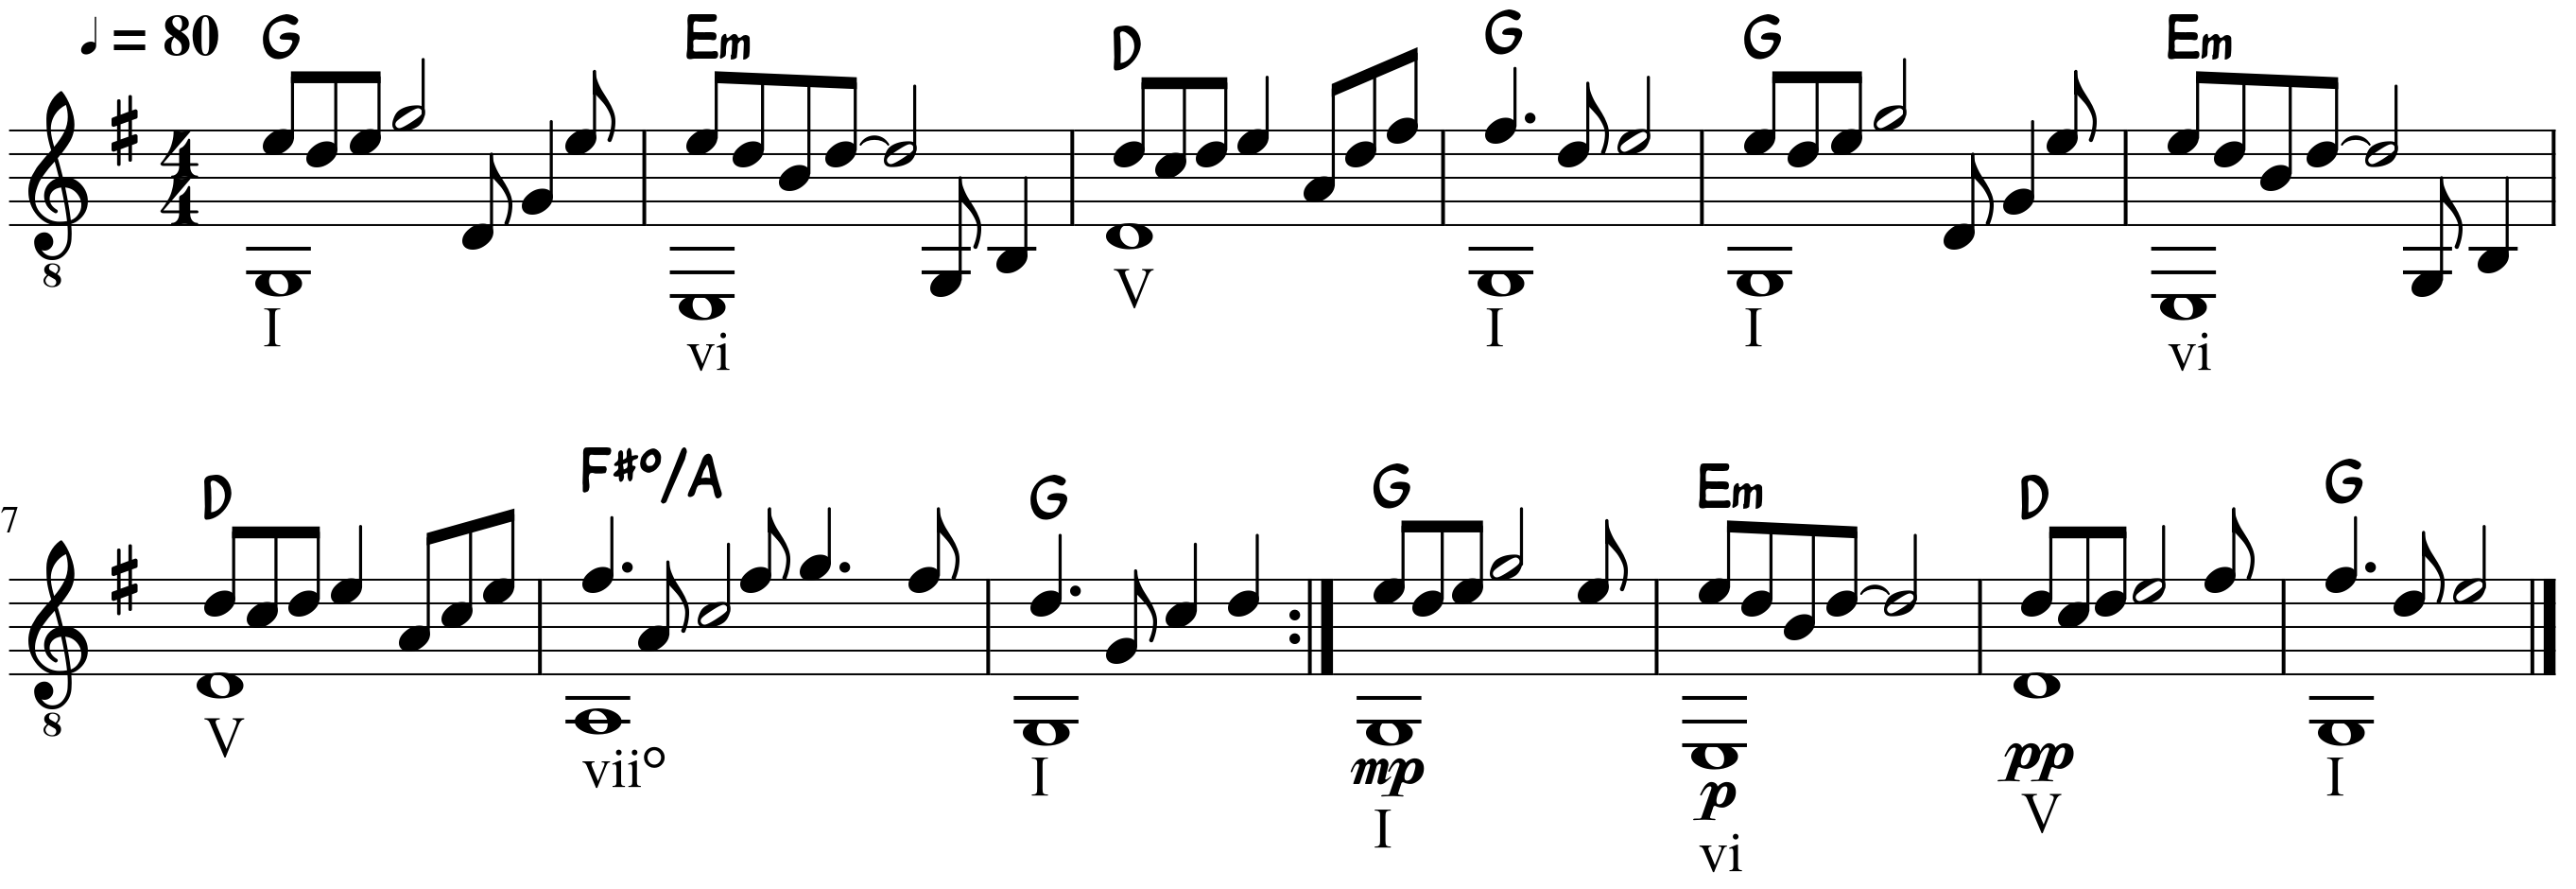
\includegraphics[width=\linewidth]{Dia_de_la_Fugaceta_Estrellada2}

\end{document}